\documentclass[addpoints]{exam}

\usepackage{epic,array,ecltree,url}
\usepackage[nointegrals]{wasysym}

\usepackage{array,epsfig}
\usepackage{amsmath}
\usepackage{amsfonts}
\usepackage{amssymb}
\usepackage{amsxtra}
\usepackage{amsthm}
\usepackage{../mlextra} % must be below ams packages
\usepackage{mathrsfs}
\usepackage{color}
\usepackage{array}
\usepackage{graphicx}
\graphicspath{ {../../art/} }
\usepackage{bm}
\usepackage{tikz}
\usepackage{multicol}

%Pagination stuff.
\setlength{\topmargin}{-.3 in}
\setlength{\oddsidemargin}{0in}
\setlength{\evensidemargin}{0in}
\setlength{\textheight}{9.in}
\setlength{\textwidth}{6.5in}

\newcommand{\tf}[1][{}]{%
\fillin[#1][0.25in]%
}


\pointsinmargin
\begin{document}


\noindent
\begin{tabular*}{\textwidth}{l @{\extracolsep{\fill}} r @{\extracolsep{6pt}} l}
{\large CS3001: Foundations of Computer Science} &  \makebox[3in]{\large Name:\enspace\hrulefill}\\
{\large April 29, 2019} & \\
{\large Exam 1} & 
\end{tabular*}\\

\fbox{\fbox{\parbox{6in}{\textbf{Instructions}: Please answer the questions 
  below to the best of your ability. Be sure to show your work where appropriate. 
   This exam is closed book, closed notes, closed computer. There are \numpoints\ 
   points in total. }}}\\
\begin{questions}

\question For each function below, indicate whether the function is injective,
  surjective, neither, or both (select only one).
\begin{parts}
\part[2] $f: \{1,2,3\} \to \{1,4,9\}$, $f(x) = x^2$. 

\begin{oneparcheckboxes}
\choice injective 
\choice surjective 
\choice neither 
\choice both (bijective) 
\end{oneparcheckboxes}

\vspace{5mm}
\part[2] $f: \N \to \N$, $f(x) = x + 1$. 

\begin{oneparcheckboxes}
\choice injective 
\choice surjective 
\choice neither 
\choice both (bijective) 
\end{oneparcheckboxes}

\vspace{5mm}
\part[2] Let $\Sigma$ be some alphabet and consider the function $f: \Sigma^+
\to \Sigma$, where $c \in \Sigma$ and we define $f(x) = c$ if there is some $y
\in \Sigma^*$ such that $cy = x$. 

\begin{oneparcheckboxes}
\choice injective 
\choice surjective 
\choice neither 
\choice both (bijective) 
\end{oneparcheckboxes}
\end{parts}
\vspace{8mm}

\question[4] Let $\Sigma = \{a,b\}$ and let $R$ be an equivalence relation on $\Sigma^*$. 
Which of the following statements \emph{must} be true? Choose all that apply.

\begin{checkboxes}
\CorrectChoice If $(ab, ba) \in R$ then $(ba,ab) \in R$.
\CorrectChoice If $(abb,bba) \in R$ and $(bba,bab) \in R$, then $(abb,bab) \in R$.
\CorrectChoice If $(abb,bba) \in R$ then $[abb]_R \cap [bba]_R = [abb]_R$.
\CorrectChoice $(a,a) \in R$.
\end{checkboxes}

\vspace{8mm}
\question[5]
Let $S$ be a set with at least one element and let $R$ be a partial order on $S$. 
Which of the following statements \emph{must} be true? Choose all that apply.

\begin{checkboxes}
\CorrectChoice If $(x,y) \in R$ and $(y,x) \in R$ then $x = y$. 
\CorrectChoice If $x = y$ then $(x,y) \in R$ and $(y,x) \in R$. 
\choice If $(x,y) \in R$ and $(x,z) \in R$ then $(y,z) \in R$. 
\choice $R$ is not symmetric. 
\CorrectChoice $R \neq \emptyset$.
\end{checkboxes}

\vspace{5mm}
\fbox{\fbox{\parbox{6in}{\textbf{Helpful Facts}: 

Let $R$ be a binary relation on $S$.
\begin{itemize}
\item $R$ is \emph{reflexive} if and only if $R(x,x)$ for all $x \in S$.

\item $R$ is \emph{symmetric} if and only if $R(x_1,x_2)$ implies $R(x_2,x_1)$.

\item $R$ is \emph{antisymmetric} if and only if $(x_1,x_2) \in R$ and $(x_2,x_1) \in
R$ implies $x_1 = x_2$.

\item $R$ is \emph{transitive} if and only if $R(x_1,x_2)$ and $R(x_2,x_3)$ implies $R(x_1,x_3)$.

\end{itemize}

Let $f$ be a function mapping from set $A$ to set $B$.

\begin{itemize}
\item $f$ is injective if and only if $f(x) = f(y) \implies x = y$ for all $x,y \in A$.

\item $f: A \to B$ is surjective if and only if for all $y \in B$ there
exists $x \in A$ such that $f(x) = y$. 
\end{itemize}}}}\\





%\question[6] True or false.
%\part \tf[T} (T/F) Let $R$ be a relation 


%\question[3] Let $S = \{a^{2k} | k \in \N_0 \}$ and let $T = \{a^{4k} | k \in
%\N_0\}$. Prove $T \subseteq S$.
%\vspace{25mm}

%\question[3] Let $K$ be a set containing \emph{all} strings of even length over the 
%alphabet $\Sigma = \{a,b\}$.  Give a Post system for $K$.
%\vspace{25mm}
%
\clearpage
\question\label{q:plpost} Answer the questions below with reference to the following Post
system: 
\begin{tabbing}
{\bf R2}XX \=  \kill
{\bf B1} \>
        \(\begin{array}[t]{l}
        p \in A
        \end{array}\) \\[2ex]
{\bf B2} \>
        \(\begin{array}[t]{l}
        q \in A
        \end{array}\) \\[2ex]
{\bf R1} \>
        \(\begin{array}[t]{l}
        x \in A \;\;\;y \in A \\
        \hline
        (x \lor y) \in A
        \end{array}\) \\[2ex]
{\bf R2} \>
        \(\begin{array}[t]{l}
        x \in A \\
        \hline
        (\ngg x) \in A
        \end{array}\) 
\end{tabbing}
\begin{parts}
\part[2] What is the derivation height of $ ((\ngg p) \lor q)$?
\vspace{10mm}
\part[3] Prove $((p \lor q) \lor (\ngg q)) \in A$.
\vspace{25mm}
\end{parts}

\question Again referring to the Post system in question \ref{q:plpost}, above, suppose
you are asked to prove the following theorem:
\textbf{``All strings in $A$ have an even number of parentheses.''}

\begin{parts}
\part[3] Which of the following induction rules is most suitable for this proof?

\begin{choices}

\choice 
	\(\begin{array}[t]{l}
	S(i) \;\lor\; \forall k \leq i.\;S(i)\;\wedge\;S(i+k)\;\lor\cdots\lor\;S(n) \Rightarrow S(n+1) \\
	\hline
	\forall n \leq i. \; S(n)
	\end{array}\)

\choice 
	\(\begin{array}[t]{l}
	S(i) \;\wedge\; S(i+1)\;\wedge\cdots\wedge\;S(j)\;\wedge\; \\
\forall n \geq j.\;S(i)\;\wedge\;S(i+1)\;\wedge\cdots\wedge\;S(n) \Rightarrow S(n+1) \\
	\hline
	\forall n \geq i. \; S(n)
	\end{array}\) 

\choice 
	\(\begin{array}[t]{l}
	S(i) \;\wedge\; \forall n \geq i.\;S(i)\;\wedge\;S(i+1)\;\wedge\cdots\wedge\;S(n) \Rightarrow S(n+1) \\
	\hline
	\forall n \geq i. \; S(n)
	\end{array}\)

\choice 
	\(\begin{array}[t]{l}
	S(i) \;\wedge\; \forall n \geq i.\;S(n) \Rightarrow S(n+1) \\
	\hline
	\forall n \geq i. \; S(n)
	\end{array}\) 
\end{choices}
\part [2] Briefly justify your answer to part (a):
\vspace{15mm}

\part[2] Write out $S(n)$. Make sure it's clear what you are parameterizing
over.
\vspace{10mm}

%\part[3] Prove the base case or base cases.
%\vspace{25mm}
%
\part[1] Let $\Sigma$ be the alphabet of $A$ and define $P$ as the set of all
string in  $\Sigma^*$ that have an even number of parentheses. Does the theorem
above claim soundness or completeness with respect to $P$?
\vspace{10mm}

\part[2] What is $\Sigma$? Give an explicit definition (i.e., write out the
    elements).
\vspace{10mm}

\end{parts}
\clearpage
\question The following Post system describes extended binary trees:

\begin{tabbing}
{\bf R2}XX \=  \kill
{\bf B} \>
        \(\begin{array}[t]{l}
        \id{nil}\in\id{RTL}
        \end{array}\) \\[2ex]
{\bf R1} \>
        \(\begin{array}[t]{l}
        l\in\id{RTL} \\
        \hline
        \id{node}(l)\in\id{RT}
        \end{array}\)\\[2ex]
{\bf R2} \>
        \(\begin{array}[t]{l}
        t\in\id{RT}\\
        \hline
        \id{cons}(t,\id{nil})\in\id{RTL}
        \end{array}\) \\[2ex]
{\bf R3} \>
        \(\begin{array}[t]{l}
        t\in\id{RT}\;\;\;u\in\id{RT} \\
        \hline
        \id{cons}(t,\id{cons}(u,\id{nil}))\in\id{RTL}
        \end{array}\) 
\end{tabbing}

\begin{parts}
\part[5] Evaluate the implications below. Write $T$ if the implication is
logically correct, $F$ otherwise.
\begin{subparts}
\subpart \tf[T] (T/F) If $l \in RTL$ has derivation height $0$, then $|l| = 0$.
\subpart \tf[T] (T/F) If $l \in RTL$ has derivation height $2$, then the number of edges
in $l$ is $0$.
\subpart \tf[F] (T/F) If $t \in RT$ has derivation height $1$, then it contains
a single edge.
\subpart \tf[F] (T/F) If $l \in RTL$ has derivation height $4$ and was formed
by rule $R3$, then it contains at least four nodes.
%\subpart \tf[T] (T/F) If $t \in RT$ has derivation height $1$, then the number of nodes 
%in $t$ is $1$.
\subpart \tf[T] (T/F) If $t \in RT$ has derivation height $2$, then the number of nodes 
in $t$ is $4$.
\end{subparts}

\part[4] Draw the structure produced in the following derivation:\\

\begin{tabular}{llllll}
$\bid{B}$  & $\id{nil} \in \id{RTL}$                                           & $\bid{B}$  & $\id{nil} \in \id{RTL}$           & $\bid{B}$  & $\id{nil} \in \id{RTL}$             \\ \cline{2-2}\cline{4-4}\cline{6-6}
$\bid{R1}$ & $\id{node}(\id{nil}) \in \id{RT}$                                 & $\bid{R1}$ & $\id{node}(\id{nil}) \in \id{RT}$ & $\bid{R1}$ & $\id{node}(\id{nil}) \in \id{RT}$   \\ \cline{2-2}\cline{4-6}
$\bid{R2}$ & $\id{cons}(\id{node}(\id{nil}), \id{nil}) \in \id{RTL}$           & $\bid{R3}$ & \multicolumn{3}{l}{$\id{cons}(\id{node}(\id{nil}), \id{cons}(\id{node}(\id{nil}),nil)) \in \id{RTL}$}   \\ \cline{2-2}\cline{4-6}
$\bid{R1}$ & $\id{node}(\id{cons}(\id{node}(\id{nil}), \id{nil})) \in \id{RT}$ & $\bid{R1}$ & \multicolumn{3}{l}{$\id{node}(\id{cons}(\id{node}(\id{nil}), \id{cons}(\id{node}(\id{nil}),nil))) \in \id{RT}$}  \\ \cline{2-6}
$\bid{R2}$ & \multicolumn{5}{l}{$\id{cons}(\id{node}(\id{cons}(\id{node}(\id{nil}), \id{nil})), \id{cons}(\id{node}(\id{cons}(\id{node}(\id{nil}), \id{cons}(\id{node}(\id{nil}),nil))), nil)) \in \id{RTL}$}  
\end{tabular}
\vspace{40mm}
\end{parts}

\question[3] Let $L$ be a set containing \emph{all} strings of odd length over the 
alphabet $\Sigma = \{a\}$. Draw an automaton that accepts all and only the
strings in $L$.
\vspace{25mm}
%

%\question Let $L$ be the language of strings accepted by the automaton
%described in the state diagram below.
%
%\begin{center}
%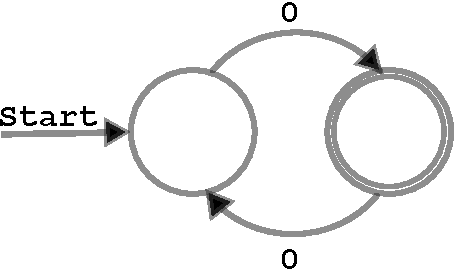
\includegraphics[width=2.5in, height=.75in,keepaspectratio=true]{oddzeroautomaton.pdf}
%\end{center}     
%\begin{parts}
%\part[1] What is the alphabet of $L$?
%\vspace{10mm}
%
%\part[2] Give a set comprehension for $L$. 
%\vspace{10mm}
%\end{parts}
%
%\question Let $\sim$ be a relation on $\Sigma = \{0,1\}$, where $x\sim y$ for $x,y \in
%\Sigma$ if and only if it is not the case that $x = 0$ and $y = 1$. 
%
%\begin{parts}
%\part[3] We claim that $\sim$ is a partial order on $\Sigma$. What properties
%of $\sim$ must be established to prove this claim is true?
%
%\vspace{10mm}
%
%\part[3] Prove that $\sim$ is transitive. 
%
%\vspace{30mm}
%
%\end{parts}
%\question
%Let $\Sigma = \{0,1,2\}$.  Let $T = \{t \in \Sigma^* | |t| \geq 3\}$.
%Now define $Z$ to be a relation on $T$ such that $xZy$ for $x,y \in T$ if and only if 
%there exist strings $r,s,m \in \Sigma^*$ such that $|m| = 3$ and $x = rm$ and $y = sm$. 
%
%\begin{parts}
%\part [3] We claim that $Z$ is an equivalence class on $T$. What properties of
%$Z$ must be established to prove this claim is true?
%\vspace{10mm}
%\part [2] Assume the claim is proven. How many equivalence classes are there with respect to $Z$?
%\vspace{10mm}
%\end{parts}
%
\clearpage
\question Let $L$ be the language of strings accepted by the automaton
described in the diagram below, and let $R$ and $Q$ be sets defined by
the Post system given on the right.

\begin{multicols}{2}
\begin{center}
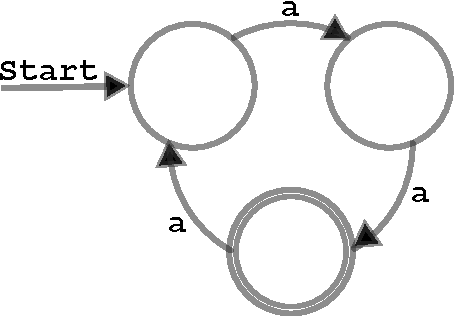
\includegraphics[width=2.5in, height=1in,keepaspectratio=true]{2mod3automaton.pdf}

\end{center}

\begin{tabbing}
{\bf R2}XX \=  \kill
{\bf B} \>
        \(\begin{array}[t]{l}
        aa \in R
        \end{array}\) \\[2ex]
{\bf R1} \>
        \(\begin{array}[t]{l}
        x\in R  \\
        \hline
        xa \in Q
        \end{array}\) \\[2ex]
{\bf R2} \>
        \(\begin{array}[t]{l}
        x\in R\;\;\;y\in Q \\
        \hline
        xy \in R
        \end{array}\) 
\end{tabbing}
\end{multicols}

%Consider the claim that $L = \{a^{3k +1} | k \in
%\N_0 \}$.  Suppose you are asked to prove that the automata accepts \emph{all}
%strings in $L$ by induction on $k$.\\
\begin{parts}
\part[3] Write out the three shortest strings contained in the set $R$.
\vspace{15mm}

\part[3] Give a set comprehension for $L$. 
\vspace{15mm}

\part[3] We claim that if a string in $R$ has derivation height $n$, it is accepted
by the automaton. Prove this claim holds for $n=0$.
\vspace{30mm}

\part We claim that if a string in $Q$ has a derivation height $n$, this string 
will put the automaton in the start state.  
\begin{subparts} 
\subpart[5] Prove this claim holds for $n=1$.
\vspace{30mm}
\subpart[3] Does the claim hold for $n=0$? Justify your answer.
\vspace{15mm}
\end{subparts} 

%\part[3] Suppose you are asked to prove, by induction on derivation height, that
%all strings in $R$ are accepted by the automaton (i.e, $R \subseteq L$).  
%Which of the following induction rules should you choose?
%\begin{choices}
%
%\choice 
%	\(\begin{array}[t]{l}
%	S_1(i)\;\wedge\;S_2(i)\;\wedge\;\forall n \geq i.\;S_1(n)\;\wedge\;S_2(n)\Rightarrow S_1(n+1)\;\wedge\;S_2(n+1)\\
%	\hline
%	\forall n \geq i. \; S_1(n)\;\wedge\;S_2(n)
%	\end{array}\) % \\[2ex]
%
%\choice 
%	\(\begin{array}[t]{l}
%	S_1(i) \;\wedge\;S_2(i) \;\wedge\; \forall n \geq i.\;S_1(i)\;\wedge\;S_2(i)\;\wedge\cdots\wedge\;S_1(n)\;\wedge\;S_2(n)\Rightarrow S_1(n+1)\;\wedge\;S_2(n+1)\\
%	\hline
%	\forall n \geq i. \; S_1(n)\;\wedge\;S_2(n)
%	\end{array}\)
%
%\choice 
%	\(\begin{array}[t]{l}
%	S(i) \;\wedge\; \forall n \geq i.\;S(n) \Rightarrow S(n+1) \\
%	\hline
%	\forall n \geq i. \; S(n)
%	\end{array}\) % \\[2ex]
%
%\choice 
%	\(\begin{array}[t]{l}
%	S_1(i) \;\wedge\; S_2(i)\;\wedge\;S_1(i+1) \;\wedge\; S_2(i+1)\;\wedge\;\cdots\wedge\;S_1(j)\;\wedge\;S_2(j) \\
%\forall n \geq
%j.\;S_1(i)\;\wedge\;S_2(i)\;\wedge\cdots\wedge\;S_1(n)\wedge\;S_2(n)\Rightarrow S_1(n+1)\wedge\;S_2(n+1)\\
%	\hline
%	\forall n \geq i. \; S_1(n)\;\wedge\;S_2(n)
%	\end{array}\) % \\[2ex]
%
%
%\end{choices}
%\part[2] Briefly justify your answer to part (a):
%\vspace{160mm}
%
\end{parts}


%Prove injective / surjective.
%Prove a partial order.
%Prove an equivalence relation.
%Give a Post System.
%Prove an element is in a Post system.
%
%Read a derivation and describe the object.
%Prove a property of full binary trees or extended binary trees.
%Read a proof and choose the correct induction rule.



%\newpage

\end{questions}
\end{document}


